A photoconductive antenna (PCA) is a semiconductor device that acts as an optical switch by increasing its conductivity when illuminated. such devices are also called photoconductors. 
Photoconductors are semiconductor devices with a direct band-gap. These devices are operated with lasers and are based on the principle of photomixing. Two interfering laser beams forming an optical beat signal are focused on the photoconductor. When the beat signals energy level is higher than that of the semiconductors band-gap energy, free electron-hole pairs are photo-generated. A bias voltage applied on electrodes of the device separates the carriers to create a displacement current. The current oscillates with the envelope of the absorbed laser light. It results in a THz signal \cite{nandiErAsInAlGaAsPhotoconductors2021}. 

The Thz signal is emitted or detected by PCAs. PCAs usually consist of a photomixing device sitting in between the antenna's electrodes. The electrodes help emit or detect the THz signal. The mathematics for THz generation through photomixing are given in the following sections.

\subsection{Principles of Photomixing for pulsed Operation}
To explain pulsed operation for THz-TDS, continuos wave (CW) operation (see figure \textbf{ABB einfügen}) is explained beforehand for easier comprehension. This chapter is mainly a review of \cite{nandiErAsInAlGaAsPhotoconductors2021,faridiPulsedFreeSpace2023,preuPrinciplesTHzGeneration2015}.

\subsubsection{CW operation}
CW THz radiation is generated using two CW lasers. The lasers have a difference frequency of $\omega_L = \omega_0 \pm \omega_{THz}$. The photon energy of the lasers has to be higher the band-gap energy of the photoconductor material: $h\nu_L > E_G$, 
where $\nu_L = \omega_L / 2\pi$, $h$ is Planck’s constant and $E_G$ is the bandgap energy of the material. The two laser signals are heterodyned (frequency mixed) using a fiber coupler before they are fed into the photoconductor with an optical field of

\begin{equation}
	\vec{E}(t) = \vec{E}_1(t) + \vec{E}_2(t) = \vec{E}_{1,0}e^{i(\omega_L - \omega_{THz}/2)t} + \vec{E}_{2,0}e^{i(\omega_L + \omega_{THz}/2)t - i\phi},
\end{equation}
where $\phi$ is the phase difference of the laser signals. The optical intensity of the absorbed laser power is given by 
\begin{equation}
	I_L(t) \sim |\vec{E}(t)|^2 = |\vec{E}_{1,0}(t)|^2 + |\vec{E}_{2,0}(t)|^2 + 2|\vec{E}_{1,0}(t) \cdot \vec{E}_{2,0}(t)|\cos(\omega_{THz}t + \phi), 
\end{equation}

which can be rewritten in terms of laser power as 

\begin{equation}
	P_L(t) = P_1 + P_2 + 2\sqrt{P_1 P_2}\cos(\beta)\cos(\omega_{THz}t + \phi), 
\end{equation}

where $\beta$ is the angle between the polarization of the electric fields. In an ideal photoconductor all laser light is absorbed. This yields in an ideal photocurrent 
\begin{equation}
	I_{Ph}^{Id}(t) = \frac{eP_L(t)}{h\nu_L} = \frac{e(P_1+P_2)}{h\nu_L} + 2\frac{e\sqrt{P_1P_2}}{h\nu_L}\cos(\beta)\cdot\cos(\omega_{THz}t + \phi).
	\label{eq_iph}
\end{equation}

We see that the ideal photocurrent $I_{Ph}^{Id}(t)$ consists of a DC component $I_{DC}^{Id}$ and an AC component $I_{THz}^{Id}$.
The DC component is given by 
\begin{equation}
	I_{DC}^{Id} = \frac{e(P_1+P_2)}{h\nu_L}.
\end{equation} 
The AC component of the ideal photocurrent is given by the expression
\begin{equation}
	I_{THz}^{Id}(t) = 2\frac{e\sqrt{P_1P_2}}{h\nu_L}\cos(\beta)\cdot\cos(\omega_{THz}t + \phi).
\end{equation}

To maximize the THz output, the AC part of the photocurrent has to be maximized. We see that $I_{THz}^{Id}$ is at its maximum when $P_1 = P_2 = P_L = P_{tot} / 2$ and $\beta = 0$. This is equivalent to identical power and polarization of the two laser signals. With these assumptions the amplitude of the ideal photocurrent's THz part becomes $I_{THz}^{Id} = eP_{tot} / (h\nu) = I_{DC}^{Id} = I^{Id}$. Ultimately inserting our assumptions into \ref{eq_iph} we get 
\begin{equation}
	I_{Ph}^{Id} = I^{Id}[1 + \cos(\omega_{THz}t + \phi)].
	\label{eq8}
\end{equation}

The generated photocurrent is usually fed into an antenna. This antenna is fabricated on the same semiconducting material as the photomixing device. The antenna shows a radiation resistance $R_A$, yielding in the ideal emitted THz power 
\begin{equation}
	P_{THz}^{Id}=\frac{1}{2}R_A (I_{THz}^{Id})^2.
	\label{eq_thz_pow}
\end{equation}

\subsubsection{Pulsed Operation}

For pulsed operation, the semiconductor absorbs a short optical pulse. The photocurrent generated by this pulse results in THz radiation when fed into an antenna e.g. The emitted THz field is proportional to the time derivative of the photocurrent generated by the lasers \cite{preuTunableContinuouswaveTerahertz2011}:
\begin{equation}
	E_{THz} \propto \frac{\partial I_{Ph}(t)}{\partial t}.
\label{eq1}
\end{equation}

The CW generation of THz radiation can be extended to the pulsed approach. Under pulsed operation multiple laser frequencies are mixed to form a single laser pulse denoted by 
\begin{equation}
	\vec{E}(t) = \sum_j^n \vec{E}_je^{i(\omega_j t + \phi j)}.
\label{eq3}
\end{equation}
Here, $\omega_j = 2 \pi \nu_j$ are the angular frequency components of each electrical field $\vec{E}_j$ and $\phi_j$ are the corresponding phase components. Assuming a typical mode locked femtosecond laser we get the following properties: 
\renewcommand{\labelenumi}{\alph{enumi})}
\begin{enumerate}
	\item The frequency components are equally spaced in the spectral domain: $\nu_j - \nu_{j-1} = R_p$. $R_p$ is the repetition rate of the laser.
	\item The phase has a fixed relationship that is linear: $\phi_j - \phi_{j-1} = const.$
\end{enumerate}

The mode locking allows for very short laser pulses in the femtosecond range.

To obtain the ideal frequency spectrum of the emitted THz field, the signal has to be Fourier transformed. Fourier transforming eq. \eqref{eq1} yields

\begin{equation}
	E_{THz}(\omega) \propto \mathcal{F}\left\{ \frac{\partial I_{Ph}(t)}{\partial t} \right\} = i\omega I_{Ph}(t), 
\end{equation}

where $\mathcal{F}\{\cdot \}$ denotes the Fourier transform and $I_{Ph}(\omega)$ is the spectrum of the photocurrent. Ideally, the spectrum of the photocurrent is proportional to the spectral width of the photocurrent. Note that the spectral width $\Delta \omega$ is inversely proportional to the temporal width $\Delta \tau$, resulting in $\Delta \omega \Delta \tau = 0.5$ The optical pulse duration must be shorter than the period of the maximum THz frequency to be obtained. 

To derive the emitted THz spectrum under pulsed operation, the details of photocurrent generation could be investigated. This however would be beyond the scope of this thesis, as exact derivative can be quite complex. Detailed derivations can be found in \cite{preuPrinciplesTHzGeneration2015}. In the following, only fundamental steps in obtaining the emitted THz field are given.

From eq. \eqref{eq1} we already know that the field generated by a radiating structure such as an antenna is proportional to the time-derivative of the current. We also know that the ideal photocurrent is proportional to the total optical power. Assuming a laser beam that shows Gaussian distributed intensity, so $\vec{E}_j$ is Gaussian distributed, eq. \eqref{eq3} becomes
\begin{equation}
	\vec{E}(t) = \vec{A}(t)e^{i\omega_Lt}.
\label{eq4} 
\end{equation}

$\vec{A}(t)$ denotes the complex envelope of the pulse while $\omega_L$ is the laser pulses central frequency. With the mode-locked laser property of a linear phase relationship, the pulse is Fourier transform-limited (bandwidth-limited), yielding an envelope of
\begin{equation}
	\vec{A}(t) = \vec{A}_0 e^{\frac{-t^2}{\tau^2}},
\end{equation}

with $\tau$ being the time domain $1/e^2$ width. This width is the difference of the two points in the Gaussian where the intensity falls to $1/e^2$. The Gaussian pulses optical intensity is once again given by
\begin{equation}
	I_L(t) \sim |\vec{E}_L(t)|^2 = I_{L,0}e^{\frac{-2t^2}{\tau ^2}}.
\end{equation} 

Note that $I_{L,0} \sim |\vec{A}_0|^2$ which corresponds to the peak intensity of the beam. 
Fourier transforming eq. \eqref{eq4} gives us the spectral components of the pulse:

\begin{equation}
	V(\nu) =  \mathcal{F}\left\{\vec{A}(t)e^{i\omega_Lt} \right\}
	= \int_{-\infty}^{+\infty}E_L(t)e^{-i2\pi\nu t}dt = |V(\nu)|e^{i\psi(\nu)}.
\end{equation}

$\psi(\nu)$ denotes the spectral phase in this case. For a Gaussian beam, the spectral intensity is given by:
\begin{equation}
	S_I(\nu) = |V(\nu)|^2 \sim \exp[-2\pi^2\tau^2(\nu - \nu_L)^2]. 
\end{equation}

The spectral $1/e^2$ width here is described by $\sigma$, with $\tau = \sqrt{2}/(\pi \sigma)$. We already know from eq. \eqref{eq_iph} that the photocurrent is proportional to the laser power, $I_{Ph}(t) \sim P_L(t)$. Thus the ideal generated photocurrent can be expressed as 

\begin{equation}
	I_{Ph}^{Id}(t) = \frac{eP_L(t)}{h\nu_L} = \hat{I}_{L,0} e^{\frac{-2t^2}{\tau^2}},
\label{eq_gauss}
\end{equation}

where $\hat{I}_{L,0}$ is the maximum generated photocurrent. From eq. \eqref{eq_gauss} we can conclude that in an ideal case, the resulting photocurrent is Gaussian distributed because the carriers respond to the lasers envelope. 

\subsubsection{Nonidealities}

The derived equations are only valid when assuming idealistic conditions. So far, nonidealities like external quantum efficiency of the semiconductor surface, intrinsic responses of the photoconductor or antenna RC roll-off losses have not been considered. A convolution approach for the derivation of these factors is introduced in \cite{preuUnifiedDerivationTerahertz2014}. The convolution approach allows for the separation of the optical spectrum and the intrinsic response of the antennas material. The overall spectrum turns out to be a product of the ideal optical spectrum and the efficiency factors or a convolution of the THz field and intrinsic properties in the time domain. Deriving these efficiency factors would be beyond the scope of this thesis. We only look at the important properties and how they influence the spectrum of our THz signal, mainly as a revision of \cite{faridiPulsedFreeSpace2023}.

In a nonideal PCA, not all laser light is perfectly absorbed. Surface reflections and finite photon absorption of the photoconductive material limit the conversion of photons to charge carriers. External quantum efficiency measures the ratio of generated charge carriers to the incident laser power. The external quantum efficiency is given by 
\begin{equation}
	\eta_{ext} = (1-R)(1-e^{-\alpha d}). 
	\label{eq_eta_ext}
\end{equation}

$R$ denotes the reflection coefficient and $\alpha$ is the absorption coefficient of the material. The thickness of the material $d$ is also taken into account. As a result combining eq.~\eqref{eq_eta_ext} eq.~\eqref {eq_gauss} the photocurrent becomes $I_{Ph}(t) = I_{Ph}^{Id}(t) \cdot \eta_{ext}$. In terms of THz power, applying eq. \eqref{eq_thz_pow}, this can be expressed as  
\begin{equation}
	P_{THz}(\omega) = P_{THz}^{Id} \cdot \eta_{ext}^2 = \frac{1}{2}R_A (I_{Ph}^{Id})^2(\omega)\eta_{ext}^2
\end{equation}

Using an anti-reflection coating decreases the materials reflectivity $R$ and increases the materials photon absorption $\alpha$. When additionally increasing the materials thickness $d$ , values of $\eta_{ext} \approx 1$ can be reached. Note that typically $\eta_{ext} < 1$. 

\begin{figure}[ht]
	\centering
	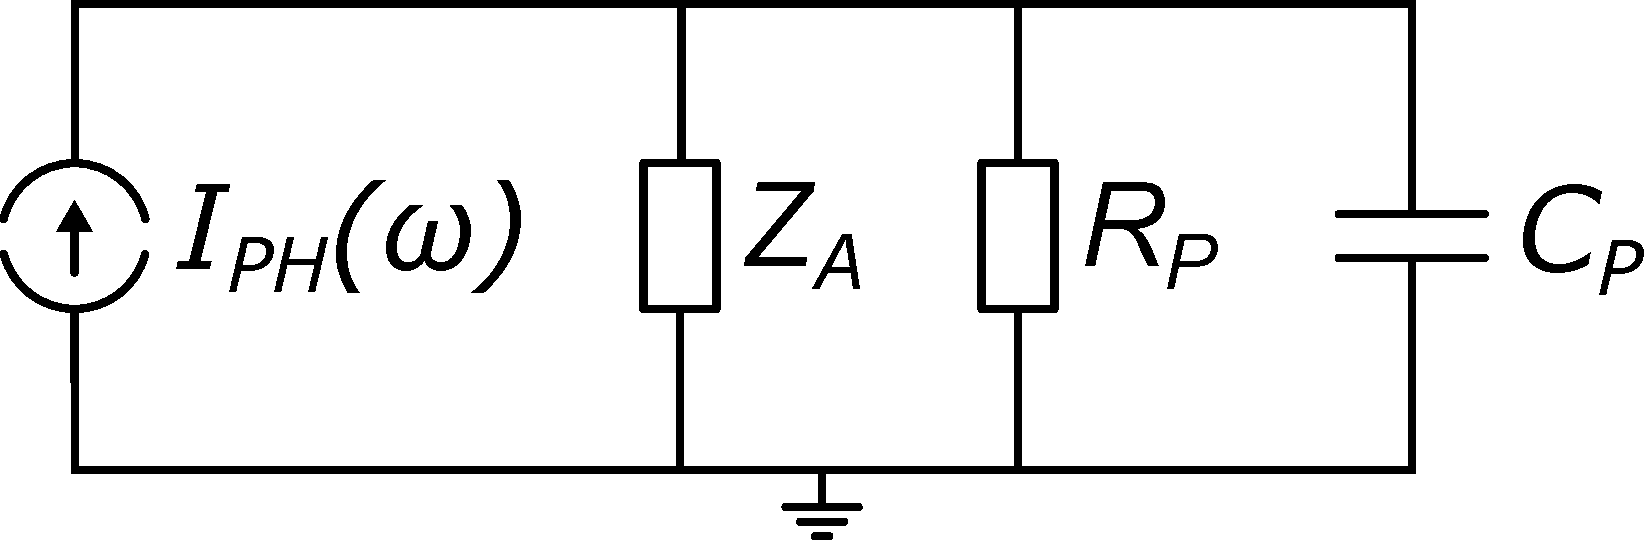
\includegraphics[width=0.7\textwidth]{figures/eq_circuit_PCA.pdf}
	\captionsetup{width=\textwidth}
	\caption{Equivalent circuit for a PCA, consisting of the antenna impedance $Z_A(\omega) = R_A + iB_A(\omega)$, the photoconductive resistance $R_P$ and the photoconductive capacitance $C_P$. The current source $I_Ph(\omega)$ models the generated photocurrent.}
	\label{PCA_eq}
\end{figure}


Two roll-off factors further decrease the emitted THz power, especially at higher frequencies. RC roll-off reflects the influence of the PCAs capacitance and impedance. A PCAs equivalent circuit \cite{fernandezolveraInternationalSystemUnits2019,collinLimitationsTheveninNorton2003} is shown in figure~\ref{PCA_eq}.

The current source $I_{Ph}(\omega)$ models the radiating element of the antenna. In parallel to the radiating element sits the devices capacitance $C_P$ between the antennas electrodes. The resistance $R_P$ describes the photoconductivity $R_P^{-1} = G_P$ in parallel to the radiation resistance of the antenna $R_A$. Not all energy is radiated, some is stored in the susceptance $B_A(\omega)$. For simplicity, the radiation impedance is modelled as purely ohmic, leaving only $R_A$. As normally $R_{P} >> R_A$, the photoconductive resistance can be neglected.  With the made simplifications, the equivalent circuit represents a typical RC circuit in low-pass filter configuration. At higher frequencies, output power is expected to decrease. The current reaching the antenna is reduced by a factor $(1 + i2\pi \nu_{THz}\tau_{RC})^{-1}$, as can be shown by calculating the transfer function of the simplified equivalent circuit: 

\begin{equation}
    H = \frac{Z_{out}}{Z_{in}} = \frac{\frac{1}{i\omega C_P}}{R_A + \frac{1}{i\omega C_P}} = \frac{1}{1 + i\omega R_A C_P} = \frac{1}{1 + i 2\pi \nu_{THz} \tau_{RC}}.    
\end{equation}

The factor by which output power will decrease is given by 

\begin{equation}
    \eta_{RC}(\nu_{Thz}) = \frac{1}{1+ (\nu_{THz}/\nu_{RC})^2} = |H|^2,  \qquad  \nu_{RC} = \frac{1}{2\pi\tau_{RC}} = \frac{1}{2\pi R_A C_P},
\end{equation}
where $f_{RC}$ is the RC 3 dB frequency.

Not all electron-hole pairs generated by photon absorption contribute to the photocurrent. A portion of charge carriers are trapped and recombine before reaching the electrodes. Due to recombination, the number of available charge carriers for photocurrent generation decreases exponentially over time. From eq. \eqref{eq8}, the average photocurrent over the transit time $\tau_{tr}$ can be calculated, yielding
\begin{align}
	I_{Ph}^{Id}(t) &= \frac{1}{\tau_{rec}} \int_{0}^{\infty} I^{Id}[1 + \cos(\omega_{THz}t + \phi)]e^{\frac{-t}{\tau_{rec}}}dt \notag \\
	I_{Ph}^{Id}(t) &=  I^{Id}\frac{\tau_{rec}}{\tau_{tr}}\left[
		1 + \frac{\sin(\omega_{Thz}t + \phi)}{\sqrt{1 + (\omega_{Thz} \tau_{rec})^2}}
	\right],
\end{align}
with recombination time $\tau_{rec}$. Both the time dependent THZ part and the DC part of the photocurrent are damped due to the trapping of charge carriers by a factor $g = \tau_{rec} /tau{tr}$. This factor $g << 1$ is called the photoconductive gain. The THz part of the photocurrent is further decreased by the lifetime roll-off 
\begin{equation}
	\eta_{LT}(\omega_{THz}) = \frac{1}{1 + (\omega_{THz}\tau_{rec})^2}.
\end{equation}

In combination with the photoconductive gain $g$ this yields an intrinsic photoconductive roll-off
\begin{equation}
	\eta_{PC}(\omega_{THz}) = g^2\eta_{LT}(\omega_{THz}) = \frac{g^2}{1 + (\omega_{THz}\tau_{rec})^2}.
\end{equation}
Ultimately, the actual THz power emitted by a PCA is given by 

\begin{equation}
    P_{THz}(\omega) = \frac{1}{2}R_A(I_{Ph}^{Id})^2\eta_{ext}^2\eta_{PC}(\omega)\eta_{RC}(\omega).
    \label{eq_power}
\end{equation}

Considering the nonidealities is important for understanding high frequency limitations in THz-TDS setups. The power spectrum and thus the spectrum of the photocurrent is highly influenced by the mentioned roll-off factors. Other influences are discussed later in this thesis. 


\subsection{Photoconductive Antennas for THz-TDS}
A PCA acts as an optical switch mainly using a relatively small active region. A laser beam is tightly focused onto the active region \cite{nandiErAsInAlGaAsPhotoconductors2021}. A rise in conductivity occurs when the semiconducting active region is exposed to the laser light. Photons generate free electrons and holes, increasing the number of charge carriers.

To emit or detect THz radiation, the switching in a photoconductive antenna must happen within a subpicosecond timescale. The switch-on time depends on the duration of the laser pulse. The switch-off time is mainly determined by the lifetime of photoexcited carriers in the semiconductor. Both a short laser pulse and a short carrier lifetime are essential for ultrafast switching. High carrier mobility and high breakdown voltage are also important for achieving good material performance.

Subpicosecond pulses are generated when a femtosecond laser pulse excites carriers in a biased PCA. Usually, such THz emitting PCAs (see Figure~\ref{typPCA}) consist of two metal electrodes sitting on a semiconducting substrate. The electrodes are biased via larger pads that are connected to the electrodes through a thin feeding strip. Femtosecond optical pulses with photon energy larger than the bandgap of the semiconductor generate free electron and hole pairs in between the electrodes. The DC bias creates a static electrical field. Free carriers are accelerated by the field. Simultaneously, the charge density declines because carriers in defect sites are trapped on the time scale of carrier lifetimes. The impulse current arising from the acceleration and decay of free carriers is the source of the subpicosecond pulses of electromagnetic radiation \cite{PrinciplesTerahertzScience2009}. 

\begin{figure}
	\centering
	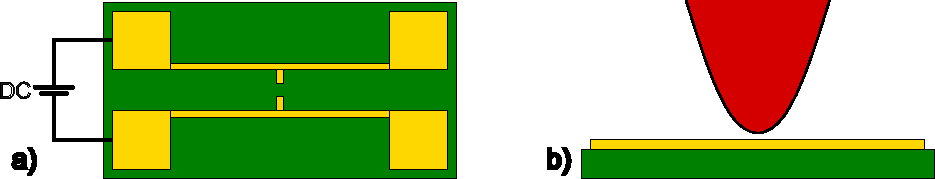
\includegraphics[width=0.9\textwidth]{figures/typiucal_PCA.pdf}
	\caption{A typical PCA is shown. a) The PCas pads are DC biased. The DC bias is fed to the antennas electrodes. b) The charge carriers in between the antennas electrodes are optically excited by a femtosecond laser pulse.}
	\label{typPCA}
\end{figure}

Typically, PCAs show a radiation resistance $R_A$ of \num{20} - \num{200} \si{\Omega}. The power and bandwidth of THz emission from a PCA vary widely depending on its topology metal electrode structure. Antenna topologies typically used in CW operation such as logarithmic periodic (log-periodic) antennas \cite{mendisTunableCWTHzSystem2004}, logarithmic spiral (log-spiral) \cite{linRoomtemperatureContinuouswaveTerahertz2025} antennas or bow-tie antennas \cite{PDFBowtieWideband} are usually not applicable in pulsed systems. 

Especially log-periodic and log-spiral antennas feature high dispersion of the THz pulse due to their long, mainly non resonant arms \cite{fernandezolveraDispersivePropertiesSelfcomplementary2017a}. As the pulse consists of multiple frequency components, the corresponding waves travel through the arms differently. Lower frequency waves are larger in wavelength. Because wavelength is proportional to wave propagation speed, the pulse is distorted because different frequency components radiate at different times. 

